\documentclass{amsart}
\usepackage{graphicx}
\graphicspath{{./}}
\usepackage{hyperref}
\usepackage{csvsimple}
\usepackage{longtable}
\usepackage{epigraph}
\title{Ethnicity Effects on Moral Views about Violence Against Others}
\author{Zulfikar Moinuddin Ahmed}
\date{\today}
\begin{document}
\maketitle

\section{Chart}

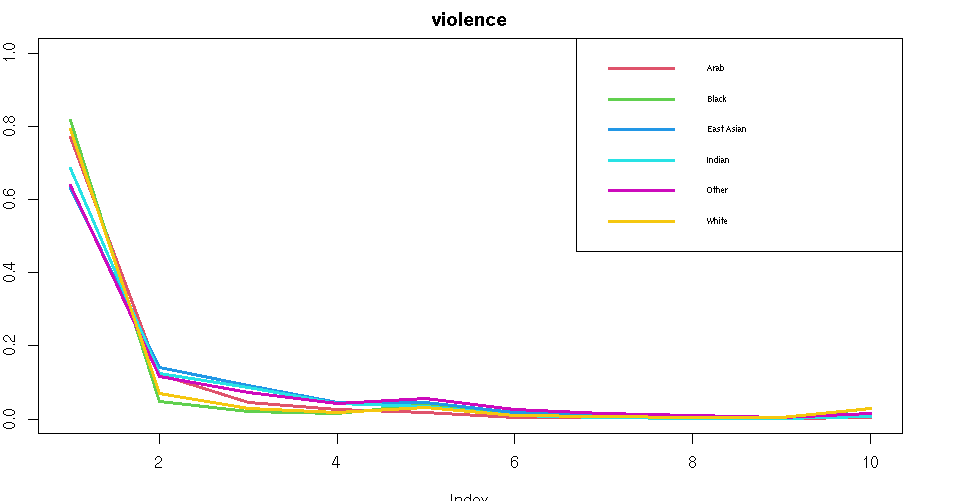
\includegraphics[scale=0.5]{ethviol.jpeg}

Let us take a look at non-violent people by ethnicity.

% latex table generated in R 4.0.3 by xtable 1.8-4 package
% Mon May 10 11:50:15 2021
\begin{table}[ht]
\centering
\begin{tabular}{rlr}
  \hline
 & eth & good \\ 
  \hline
1 & Arab & 98.08 \\ 
  2 & Black & 94.39 \\ 
  3 & East Asian & 95.28 \\ 
  4 & Indian & 97.27 \\ 
  5 & Other & 92.64 \\ 
  6 & White & 94.04 \\ 
   \hline
\end{tabular}
\end{table}

This is quite interesting because Arabs are the least violent ethnicity here, and whites are more violent than blacks.  Both f these are quite far from the racial propaganda that I find propagating in America routinely.

Regardless, the sober assessment here is that roughly 95\% of all ethnicities are peaceful people.

Now let us record the ethnicity effect on violence.

% latex table generated in R 4.0.3 by xtable 1.8-4 package
% Mon May 10 11:59:02 2021
\begin{table}[ht]
\centering
\begin{tabular}{rlr}
  \hline
 & eth & explained \\ 
  \hline
1 & Arab & 0.57 \\ 
  2 & Black & 2.05 \\ 
  3 & East Asian & 2.62 \\ 
  4 & Indian & 0.59 \\ 
  5 & Other & 1.86 \\ 
  6 & White & 1.14 \\ 
   \hline
\end{tabular}
\end{table}

\end{document}
